    %% This is file `elsarticle-template-1-num.tex',
%%
%% Copyright 2009 Elsevier Ltd
%%
%% This file is part of the 'Elsarticle Bundle'.
%% ---------------------------------------------
%%
%% It may be distributed under the conditions of the LaTeX Project Public
%% License, either version 1.2 of this license or (at your option) any
%% later version.  The latest version of this license is in
%%    http://www.latex-project.org/lppl.txt
%% and version 1.2 or later is part of all distributions of LaTeX
%% version 1999/12/01 or later.
%%
%% Template article for Elsevier's document class `elsarticle'
%% with numbered style bibliographic references
%%
%% $Id: elsarticle-template-1-num.tex 149 2009-10-08 05:01:15Z rishi $
%% $URL: http://lenova.river-valley.com/svn/elsbst/trunk/elsarticle-template-1-num.tex $
%%
%\documentclass[preprint,12pt]{elsarticle}
%\documentclass[preprint,5p, twocolumn]{elsarticle}
\documentclass[onecolumn]{elsarticle}

%% Use the option review to obtain double line spacing
%% \documentclass[preprint,review,12pt]{elsarticle}

%% Use the options 1p,twocolumn; 3p; 3p,twocolumn; 5p; or 5p,twocolumn
%% for a journal layout:
%% \documentclass[final,1p,times]{elsarticle}
%% \documentclass[final,1p,times,twocolumn]{elsarticle}
%% \documentclass[final,3p,times]{elsarticle}
%% \documentclass[final,3p,times,twocolumn]{elsarticle}
%% \documentclass[final,5p,times]{elsarticle}
%% \documentclass[final,5p,times,twocolumn]{elsarticle}

\usepackage{subcaption}
%% The graphicx package provides the includegraphics command.
\usepackage{graphicx}
%% The amssymb package provides various useful mathematical symbols
\usepackage{amssymb}
%% The amsthm package provides extended theorem environments
%% \usepackage{amsthm}

%% The lineno packages adds line numbers. Start line numbering with
%% \begin{linenumbers}, end it with \end{linenumbers}. Or switch it on
%% for the whole article with \linenumbers after \end{frontmatter}.
\usepackage{lineno}
\usepackage[colorinlistoftodos,textwidth=1.25cm,textsize=tiny]{todonotes}
\setlength{\marginparwidth}{0.9cm}

\usepackage{url}
\urlstyle{rm}

%% PACKAGE for ALIGNED
\usepackage{amsmath}
\usepackage{amssymb}

%% PAKACAGE FOR TABLES 
\usepackage{multirow}
\usepackage{colortbl}
\usepackage{rotating}

%%% PACKAGE FOR WATERMARKS
%% \usepackage{draftwatermark}


%% natbib.sty is loaded by default. However, natbib options can be
%% provided with \biboptions{...} command. Following options are
%% valid:

%%   round  -  round parentheses are used (default)
%%   square -  square brackets are used   [option]
%%   curly  -  curly braces are used      {option}
%%   angle  -  angle brackets are used    <option>
%%   semicolon  -  multiple citations separated by semi-colon
%%   colon  - same as semicolon, an earlier confusion
%%   comma  -  separated by comma
%%   numbers-  selects numerical citations
%%   super  -  numerical citations as superscripts
%%   sort   -  sorts multiple citations according to order in ref. list
%%   sort&compress   -  like sort, but also compresses numerical citations
%%   compress - compresses without sorting
%%
%% \biboptions{comma,round}

% \biboptions{}

\DeclareMathOperator*{\argmax}{arg\,max}

\journal{Expert Systems with Applications}

\begin{document}

\begin{frontmatter}

%% Title, authors and addresses

\title{Flying Tourist Problem: Flight Time and Cost Minimization in Complex Routes}

%% use the tnoteref command within \title for footnotes;
%% use the tnotetext command for the associated footnote;
%% use the fnref command within \author or \address for footnotes;
%% use the fntext command for the associated footnote;
%% use the corref command within \author for corresponding author footnotes;
%% use the cortext command for the associated footnote;
%% use the ead command for the email address,
%% and the form \ead[url] for the home page:
%%
%% \title{Title\tnoteref{label1}}
%% \tnotetext[label1]{}
%% \author{Name\corref{cor1}\fnref{label2}}
%% \ead{email address}
%% \ead[url]{home page}
%% \fntext[label2]{}
%% \cortext[cor1]{}
%% \address{Address\fnref{label3}}
%% \fntext[label3]{}


%% use optional labels to link authors explicitly to addresses:
%% \author[label1,label2]{<author name>}
%% \address[label1]{<address>}
%% \address[label2]{<address>}

\author[inescid,ist]{Rafael Marques}
\author[inescid,ist]{Lu\' is Russo}
\author[inescid,ist]{Nuno Roma}

\address[ist]{Instituto Superior T\'ecnico, Universidade de Lisboa}
\address[inescid]{INESC-ID, Rua Alves Redol, 9, 1000-029 Lisboa, Portugal}

\begin{abstract}
The Flying Tourist Problem (FTP) is formalized and addressed as a generalization of the NP-hard Traveling Salesman Problem (TSP), and whose goal is to find the best schedule, route, and set of flights, for any given unconstrained multi-city flight request. An effective methodology that allows an efficient resolution of this rather demanding problem is also proposed by considering different heuristics and meta-heuristic optimization algorithms, including the Ant Colony Optimization (ACO) and the Simulated Annealing (SA), allowing the identification of solutions in real-time, even for large instances. The implemented system was evaluated using different criteria and the obtained results show its ability to consistently present solutions that are as close as 10\% to the optimal. Furthermore, when comparing the developed system to the only known (but not-disclosed) alternative for flight search, it was shown that it provides the cheapest and the best-recommended solutions, respectively 95\% and 74\% of the times, allowing the user to save a significant amount of time and money.
\end{abstract}

\begin{keyword}
Combinatorial Optimization, Traveling Salesman Problem, Ant Colony Optimization, Simulated Annealing, Flight Search.
\end{keyword}

\end{frontmatter}


%%\linenumbers

%%___________________________________________________________
%% ________________________ MAIN ____________________________
%%___________________________________________________________

%%\SetWatermarkText{Draft}
%%\SetWatermarkScale{5}

%%%%%%%%%%%%%%%%%%%%%%%%%%%%%%%%%%%%%%%%%%%%%%%%%%%%%%%%%%%%%%%%%%%%%%%%%%%%%%%%%%%%%%%%%%%%%%%%%%%%%%%%%%%
%%%%%%%%%%%%%%%%%%%%%%%%%%%%%%%%%%%%%%%%%%%%%%%%%%%%%%%%%%%%%%%%%%%%%%%%%%%%%%%%%%%%%%%%%%%%%%%%%%%%%%%%%%%
\section{Introduction}
\label{sec:intro}
Consider a person who wants to visit $N$ different cities in the most efficient way possible. In the combinatorial optimization domain, this problem is well known as the Traveling Salesman Problem (TSP) and it is considered to be part of one of the most complex classes of problems (\cite{np_completeness}). This difficulty arrives from the exponential growth of the number of possible solutions, given approximately by $N!$. 

Upon the introduction and formalization of the TSP, this problem could simply be stated as \textit{``Given a list of N cities and the distances between them, what is the best closed tour that visits every city exactly once?''} or, as considered in the graph theory domain, \textit{``Given a complete undirected graph with weighted edges, what is the minimum cost Hamiltonian cycle?''}. This formulation has a vast number of applications and it is very useful for the majority of the routing problems that occur on a network that can be modulated as a graph (\cite{tsp_book_computation,graph_theory_book}). 

In this paper, the classic problem of traveling through $N$ different cities is revisited, but assuming the particular case applied to commercial flights transportation. This specific formulation is closely related to the generic TSP, in the sense that both problems aim to find the most efficient way to visit a given number of cities. However, there are some considerable differences. While the generic TSP (and its asymmetric variation) considers that the cost between two cities is always constant over time, such assumption is certainly not true for the case of commercial flights, as the tickets price depend not only on the date, but also on the direction of the trip (i.e., \textit{price}(${A\rightarrow B}$) $\neq$ \textit{price}(${B\rightarrow A}$)).

As a result of this time (and direction) dependency, a reasonable assumption would be to consider this as a Time-Dependent Traveling Salesman Problem (TDTSP)(\cite{tdtsp_fox_2}). Due to the specific characteristics and goals of the problem, this is, in fact, the case. However, the majority of the literature around the TDTSP makes a number of assumptions that, in many cases, do not adequately describe the problem. An example of this is the TDTSP formulation introduced by J.C.Picard (\cite{tdtsp_picard}), which considers that the waiting period in each city is exactly one time-period. Such an assumption is not always verified, not only due to existing restrictions of flight offers in such routes, but also because flying dates are also dependent on the traveler's convenience.

The observed limitations of the TDTSP formulations lead to the need of a more realistic formulation of the problem (herein referred to as the \textit{Flying Tourist Problem} (FTP)). In particular, while the goal of the TSP is to find the best \textit{route} which efficiently connects all $N$ cities, the goal of the Flying Tourist Problem is to find the best \textit{route, schedule} and \textit{set of flights} for the trip. Furthermore, the objective function of this problem must also reflect multiple objectives, particularly the total \textit{cost} and \textit{flight duration} of the trip.

To the best of the authors' knowledge, no formal solution exist to solve this specific problem. While there are several meta-search engines that are capable of responding to multi-city requests, the user must always specify a particular route and schedule. However, from the analysis of the search space perspective, such scenario corresponds to the inspection of a single solution among the $N!$ solutions to the problem. Furthermore, as the number of cities to be visited increases, finding the best set of flights rapidly becomes a slow, time consuming, and tedious process.

On the other hand, a commercial flight search application was recently launched by \textit{Kiwi} (\url{www.kiwi.com}), denoted as \textit{Nomad}. This web-service addresses the same problem as the presented work and it is currently the only (non-disclosed) tool for the resolution of this problem. Consequently, it will be treated as the state-of-the-art in the quantitative evaluation of the developed system. According to the obtained results, the presented optimization algorithm is able to provide cost and flight duration gains as high as 18\% and 24\% when compared to \textit{Kiwi}'s \textit{Nomad} implementation, when considering trips with more than 5 nodes. Even more significant gains are obtained when more nodes are considered.

With this in mind, the goals and major contributions of this work are as follows:
\begin{itemize}
  \item Formal definition of the \textit{Flying Tourist Problem} that looks for the best schedule and set of flights that visit a given list of cities, by minimizing both the total \textit{cost} and \textit{flight duration};
  \item Proposal of efficient optimization algorithms to solve the stated problem;
  \item Implementation of a system prototype capable of providing a high-quality solution for the problem (in an efficient manner) when using real-world data and resources;
  \item Analysis and evaluation of the obtained results, not only in terms of the obtained set of solutions, but also in terms of the achieved gains (time and cost).
\end{itemize}

The remaining of this article is structured as follows. Section \ref{sec:literature} presents a brief overview of the most relevant literature. This is followed by a formal definition of the problem, presented in section \ref{sec:problem}. Section \ref{sec:optimization} covers in detail the proposed optimization procedure and section \ref{sec:system} presents the architecture of the developed system prototype and the most relevant implementation details. Section \ref{sec:results} does an analysis of the obtained solutions based on several experiments and compares it to the current state-of-the-art. Finally, section \ref{sec:conclusions} presents the major conclusions and addresses possible future work directions.

%%%%%%%%%%%%%%%%%%%%%%%%%%%%%%%%%%%%%%%%%%%%%%%%%%%%%%%%%%%%%%%%%%%%%%%%%%%%%%%%%%%%%%%%%%%%%%%%%%%%%%%%%%%
%%%%%%%%%%%%%%%%%%%%%%%%%%%%%%%%%%%%%%%%%%%%%%%%%%%%%%%%%%%%%%%%%%%%%%%%%%%%%%%%%%%%%%%%%%%%%%%%%%%%%%%%%%%
\section{Literature Review}
\label{sec:literature}

The TSP is a classical formulation in several domains, including the routing and graph theories (\cite{tsp_book_computation,graph_theory_book}). It is also frequently applied in other specific optimization scenarios, including the Vehicle Routing Problem (VRP), or the single-machine scheduling. Although it usually refers to its symmetric versions, over an undirected graph,  other variations are common, based on its asymmetric counterpart over a directed graph (\cite{asymmetric}). 

The several optimization algorithms that have been proposed for the TSP are usually grouped into \textit{exact}, \textit{heuristic} and \textit{metaheuristic} approaches. 

Most of the exact algorithms (\cite{tsp_exact,vrp_exact}) rely on an Integer Linear Programming (ILP) formulation, while others are based on branch and bound (\cite{bnb_old,bnb_new}) and minimum spanning tree (\cite{trees}) techniques. However, the long execution times that characterize these approaches make them impractical in most application scenarios.

As a result, many heuristic methods to solve either the TSP (\cite{tsp_heuristics}) and the VRP (\cite{vrp_heuristics}) have been proposed. Among the most common approaches are improvement heuristics, such as the k-opt exchange (\cite{heuristics_tsp}), construction heuristics, including the nearest neighbor (\cite{tsp_exact}), and tabu search (\cite{tabu}). For the particular case of the TSP, the Lin-Kernighan heuristic (\cite{lk_alg}) is a particularly efficient algorithm. It was the state-of-the-art (for asymmetric TSPs) for over a decade. In general, its results are within 2\% of the lower bound and often generate optimal solutions (\cite{local_search_book}). Despite this, the Lin-Kernighan heuristic cannot be directly applied to the asymmetric TSP. Instead, it is necessary to apply a graph transformation, converting the asymmetric TSP into a symmetric instance, with twice as many nodes (\cite{atsp_transformation}).

For over 50 years, exact and heuristic algorithms dominated the used techniques for the resolution of combinatorial optimization problems, such as the TSP and the VRP. However, a great interest has also been devoted to the metaheuristic algorithms over the last 30 years. Metaheuristics can be seen as higher order heuristics: they take advantage of an underlying heuristic and guide the algorithm to produce an efficient search space exploration. The class of metaheuristics is vast and includes algorithms such as the Simulated Annealing (\cite{SA_1}), Genetic Algorithm (\cite{genetic}), Ant Colony Optimization (\cite{aco}), Particle Swarm Optimization (\cite{swarm}) and many more. A particular attention will be devoted to the Simulated Annealing and the Ant Colony Optimization approaches, as a result of its relation with the proposed solution.

The Ant Colony Optimization (ACO) is actually a group of several different optimization algorithms, as the Ant System (AS), Elitist AS, Ant Colony System, and min-Max AS. During the development of these algorithms, the TSP was the first optimization problem to be solved using these metaheuristics. This was primarily because the TSP served as a good benchmark test for evaluating the algorithm's performance. The first of these algorithms, the AS, did not consistently present high-quality results. However, the later algorithms (including the Ant Colony System) were capable of competing with the state-of-the-art (\cite{aco_tsp}). After fine-tuning, the ACO was rapidly applied to a vast collection of combinatorial optimization problems, as the VRP (\cite{aco_vrp}), quadratic assignment (\cite{aco_qa}), and weighted tardiness (\cite{aco_wt}), where the TSP occurs as a special case of these three problems. Recent research around the ACO metaheuristic has focused on the resolution of multi-objective combinatorial optimization problems, as presented in (\cite{aco_mo_1,aco_mo_2}).  

The evolution of the Simulated Annealing (SA) is somewhat similar to that of the ACO (although SA appeared 10 years before). It was one of the first meta-heuristic to be developed, and its success resides on its ability to escape local minimum, by performing hill-climbing techniques. Just like with the ACO, the first combinatorial optimization problem to be solved using SA was the TSP (\cite{sa_tsp}). The VRP was a natural consequence of this (\cite{sa_vrp}). There are also several works which focus on TSP and VRP with time-windows (\cite{sa_tsptw,sa_vrptw}), including real-world environments that consider that the travel times is stochastic instead of well defined (\citet{vrp_exact}), as well as several SA algorithms which focus on multi-objective optimization (\cite{sa_mo}).

Besides these two classical approaches, there are also some other proposals that apply hybrid optimization algorithms, combining two or more meta-heuristics.
An example of this is the \textit{genetic simulated annealing ant colony system} \citet{expert_mistura_de_heuristicas}.
%An example of this is the Multi-agent Simulated Annealing (\cite{sa_ma}).


%%%%%%%%%%%%%%%%%%%%%%%%%%%%%%%%%%%%%%%%%%%%%%%%%%%%%%%%%%%%%%%%%%%%%%%%%%%%%%%%%%%%%%%%%%%%%%%%%%%%%%%%%%%
%%%%%%%%%%%%%%%%%%%%%%%%%%%%%%%%%%%%%%%%%%%%%%%%%%%%%%%%%%%%%%%%%%%%%%%%%%%%%%%%%%%%%%%%%%%%%%%%%%%%%%%%%%%
\section{Flying Tourist Problem (FTP) formulation}
\label{sec:problem}

Consider a tourist who wishes to take a trip that visits every node (city) $i$ in the set of nodes $V$, $|V|$ = $N$, with no particular order. The start node will be denoted as $v_{0}$, while the return node as $v_{n+1}$, and the complete set of nodes is given by $V_c$ = $V \cup \{v_0\} \cup \{v_{n+1}\}$. The trip must start at a time $t \in T_0 = [T_{0m}, T_{0M}]$. Upon visiting a node, the tourist will stay there for a duration of $d$ time-units (days). Consider that for each node to be visited, there is a range for the value that $d$ might take, restricted as $d \in d_i = [d_{im}, d_{iM}]$ and $d_{iM} \geq d_{im} \geq 1$. The complete set of durations associated to each city is given by $D = \{ d_i | i \in V\}$, therefore $|D| = N$. Furthermore, to each city $i \in V$, there is an associated time-window $w_i$ which defines the set of dates in which the city $i$ may be visited. The set of all time windows is denoted $TW = \{w_i|i \in V\}$ and has size $N$, $|TW| = |V| = N$,

The FTP is completely defined by a structure $G = (V_c, A, T_{0}, D, TW)$, used to create a multipartite graph describing the request. This multipartite graph is divided into $k$ layers, where each layer corresponds to a particular moment in time. Besides this, every node in a layer is connected to all nodes in the subsequent layer. The set of arcs that connects these nodes is given by $A$. To each arc $a \in A$, it is associated a cost $c_{a}$ (ticket cost) and a processing time $p_{a}$ (flight duration), which depend upon the routed nodes, as well as the time in which the arc transition is initiated, that is, $\forall a_{ij}^{t} \in A$, $c_{ij}^{t} \geq 0$ and $p_{ij}^{t} \geq 0$.

A valid solution $s$ to the formulated FTP is a set of arcs (commercial flights) which start from node $v_0$ during the defined start period, visits every node $i$ in $V$ during its defined time-window $w_i$, by considering the staying durations defined by $d_i$, and finally returns to node $v_{n+1}$. The set of all valid solutions is given by $S$. The goal of the FTP is to find the global minimum $s^* \in S$, with respect to the considered objective function.

The objective function associated to this problem depends on the user criteria. While some users might consider the expended cost to be the most important factor, there are others who consider the total flight duration of crucial importance. Thus, a total of three different objective functions shall be herein considered: (i) the expended cost (see eq.~\ref{eq:obj_cost}), (ii) the flight duration (see eq.~\ref{eq:obj_time}), and (iii) a balanced cost (see eq.~\ref{eq:obj_entropy}), where the latter corresponds to a weighted sum between the former two. 
\begin{equation}
\label{eq:obj_cost}
  F_{c}(s) = \sum_{n=0}^{N+1} c(s[n])
\end{equation}

\begin{equation}
\label{eq:obj_time}
  F_{t}(s) = \sum_{n=0}^{N+1} p(s[n])
\end{equation}

\begin{equation}
\label{eq:obj_entropy}
  F_{e}(s) = \sum_{n=0}^{N+1} w_c*c(s[n]) + w_p*p(s[n])
\end{equation}

Figure \ref{fig:multipartite_sol} illustrates the multipartite graph associated to a simple instance of the FTP with $v_{n+1} = v_0 = X$, one possible start date ($t = 0$), 3 nodes to visit $(A, B, C)$, with a fixed duration of respectively (1,2,3) time-units, and no constraints relative to the time-window of each city. A possible solution to this problem instance corresponds to the set of arcs $(a_{X,B}^{0}, a_{B,A}^{2}, a_{A,C}^{3}, a_{C,X}^{6})$.

\begin{figure}[tbp]
  \centering
  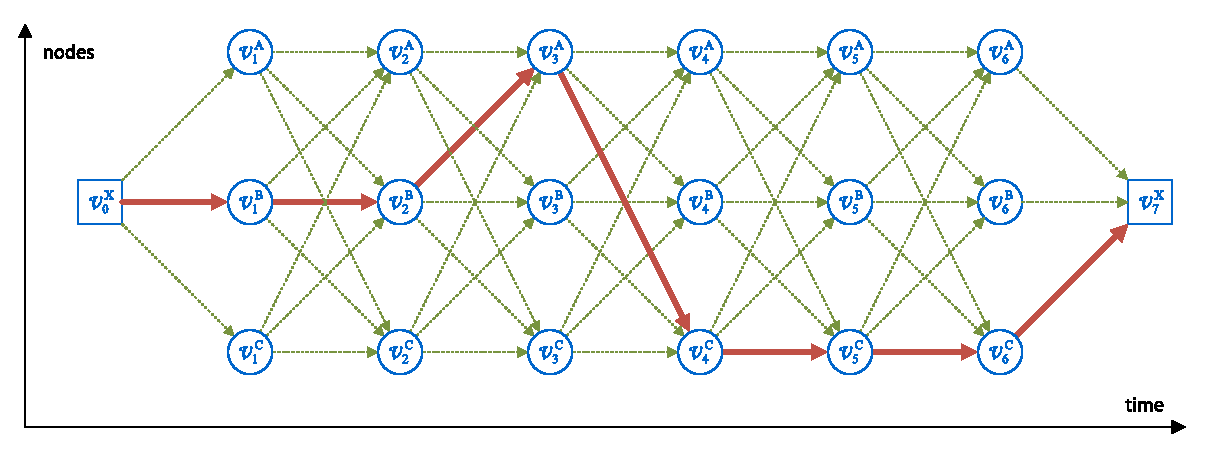
\includegraphics[width=1.0\columnwidth]{./fig1.eps}
  \caption{Illustration of a Flying Tourist Problem using a multipartite graph. To each node (A,B,C) it is associated a waiting period of respectively (1,2,3) time units. The red arrows represent a possible solution to the problem.}
  \label{fig:multipartite_sol}
  \vspace*{-0.5cm}
 \end{figure}

Despite the apparent complexity of the proposed definition, it can be used to state very simple flight searches, including one-way and round-trip flights. For example, the problem of finding a single flight from $A$ to $B$ at date $T$ can be instantiated as a FTP given by $v_0$ = $A$, $v_{n+1}$ = $B$, $T_{0} = T$, and $V$ = $D$ = $TW$ = $\{\}$. In its turn, a round-trip flight involving the same two cities and the same start date, in which the staying period in $B$ is $b$ days, is given by $v_0 = v_{n+1} = A$, $T_{0} = X$, $V = \{B\}$, $D = \{b\}$ and $TW$ = $\{\}$. Thus, this definition is adequate either for simple and complex trips, which can be customized according to the user search criteria, by setting either an extended start period, or flexible waiting periods.


\subsection{Relation to the TSP}

As previously stated, the proposed FTP is closely related to the TSP and to its time-dependent variation. Given the following list of constraints:
\begin{enumerate}
      \item $v_{n+1} = v_0$;
      \item $T_0 = 0$;
      \item $w_i = [0, +\infty[$, $\forall i \in V$;
      \item $d_i = 1$, $\forall i \in V$;
    \item $c_{ij}^{t} = c_{ij}$, $\forall i, j \in V$, $\forall t$.
\end{enumerate}
constraints (1-4) enable the reduction of the devised FTP to a TDTSP, as proposed by J.C.Picard (\cite{tdtsp_picard}), and the final constraint (5) reduces the problem to the classical TSP.

Since the FTP occurs as a generalization of the TSP, and given that the latter problem is well-known to be Np-hard complex, than so is the former one.


\subsection{Graph construction}
\label{sec:graph}

By considering the presented FTP definition, the total number of layers ($k$) of the devised multipartite graph represents the total time span between the earliest date at which the trip might start and the latest date in which it should finish. The arcs that connect those nodes are divided into three groups: \textit{initial}, \textit{transition} and \textit{final} arcs.

The \textit{initial} arcs are those which might initiate the trip. Consequently, they must start at node $v_0$, at a time $t \in T_0 = [T_{0m}, T_{0M}]$, connecting $v_0$ to every node in $V$. There are a total of $k_i = T_{0M} - T_{0m} + 1$ layers for the initial arcs.

Conversely, the \textit{final} arcs are those that connect every node in $V$ to the return node, $v_{n+1}$. There are as many final layers as there are initial layers, and the final layer extends from $T_{fm}$ to $T_{fM}$, where $T_{fm}$ = $T_{0m} + \sum(D)$ and $T_{fM}$ = $T_{0M} + \sum(D)$, where $\sum(D)$ corresponds to the summation of all entries belonging to $D$. In the example depicted in Figure~\ref{fig:multipartite_sol}, there is a single initial and final layer, since there is only one possible start date.

The \textit{transition} arcs are those which fully connect the $N$ nodes belonging to $V$. The earliest transition arc occurs at a time no sooner than $t_1 = T_{0m} + min(D)$, where $min(D)$ corresponds to the lowest entry of the set of staying durations. Hence, if the trip starts by transiting an initial arc at time $T_{0m}$, the first transition arc might only be traversed $min(D)$ time-units later. By following a similar approach, the latest transition arc can occur no latter than $t_2 = T_{0M} + \sum(D) - min(D)$. Thus, there are a total of $k_2 = t_2-t_1+1$ transition layers, and $k_2*n*(n-1)$ transition arcs.

The union of the initial, transition and final arcs gives the set $A$ of all the arcs, which may be used to construct a solution to the requested trip. 

Having the information relative to the multipartite graph associated to the devised FTP, it is now possible to construct a three-dimensional array matrix representing this problem, where each entry of the array corresponds to an arc connecting two nodes, at a particular moment in time. This weight matrix is initialized with a very high cost value (as to reject arcs which may not be part of the solution), and every entry of it is updated according to the information of the multipartite graph and the respective objective function. Finally, this weight matrix may be used as input for the optimization system (see section~\ref{sec:optimization}).

Although it is clear that any arc $a \in A$ corresponds to a particular flight, it should be noted that no specific or limiting assumption was considered up until now. Instead, it was assumed an entirely abstract arc definition, connecting two nodes at a specific moment in time. In order to transform this set of arcs into a corresponding set of flights, it is necessary to obtain real-world flight data from some external source. This will be further detailed in section~\ref{sec:system}.
%%%%%%%%%%%%%%%%%%%%%%%%%%%%%%%%%%%%%%%%%%%%%%%%%%%%%%%%%%%%%%%%%%%%%%%%%%%%%%%%%%%%%%%%%%%%%%%%%%%%%%%%%%%
%%%%%%%%%%%%%%%%%%%%%%%%%%%%%%%%%%%%%%%%%%%%%%%%%%%%%%%%%%%%%%%%%%%%%%%%%%%%%%%%%%%%%%%%%%%%%%%%%%%%%%%%%%%
\section{Optimization System}
\label{sec:optimization}

Two distinct metaheuristic algorithms were considered in the devised optimization system: the Ant Colony Optimization (ACO) and the Simulated Annealing (SA). Each FTP instance is solved with these two algorithms and the best solution is selected.


\subsection{Ant Colony Optimization}

The developed ACO algorithm receives, as input, a weight matrix with the information of the solution components of the problem. It must also receive other relevant parameters for the solution construction process, as the initial and final node and the set of waiting periods $D$. 

The initialization of the ACO metaheuristic requires the construction of an initial pheromone matrix. The initial pheromone value is set according to Eq.~\ref{eq:tau_zero}, where $n$ is the number of nodes and $C^{nn}$ is the cost of the nearest neighbor heuristic. 
\begin{equation}
\label{eq:tau_zero}
  \tau_{ij}^{t} = \tau_{0} = \frac{1}{nC^{nn}}
\end{equation}

The initialization of the metaheuristic also requires the definition of a variety of algorithm-specific parameters, such as the number of ants $m$, the pheromone evaporation rate $\rho$, the heuristic relative influence $\beta$, the pheromone relative influence $\alpha$, and the exploration rate $Q_0$. 

After the initialization, and until the termination condition is met, the algorithm enters into a iterative cycle, where every ant belonging to the colony constructs a solution to the problem. This is followed by a pheromone update phase, to reflect the colony search experience. A new iteration may only start after all ants have finished the solution construction process and the pheromone matrix has been updated.

The construction process that is undertaken by each ant is as follows. First, the current time is set to a value belonging to the allowable trip starting dates, $t \in T_0$, and the current node is set to the start node $v_0$. Each ant enters an iterative cycle until all nodes belonging to $V$ are visited. At every step of this cycle, an ant chooses a solution component by either \textit{exploiting} or \textit{exploring} the search space. The decision of exploiting or exploring depends on the algorithm parameter $Q_0$ and on a pseudo-random value $q$, calculated at runtime. The selection of the solution component $j$, which identifies the next city to be visited, is given by Eq.~\ref{eq:selection_rule}. After the selection of each solution component, it is necessary to update the time, incrementing it by the duration relative to the selected city.

\begin{equation}
  \label{eq:selection_rule}
  j =  \left \{
    \begin{aligned}
      & exploitation \ (\text{Eq.} \ \ref{eq:exploitation}) , && \text{if}\ q \leq Q_0 \\
      & exploration \ (\text{Eq.} \ \ref{eq:exploration}), && \text{otherwise}
    \end{aligned} \right. 
\end{equation}

The \textit{exploitation} of the search space utilizes the random-proportional rule, defined by Eq.~\ref{eq:exploitation}, which determines the next solution component of the ants' solution. The $J_k(i,t)$ term represents the set of solution components that might be selected to form a valid solution component by an ant in its current \textit{state}, where the state refers to the current ant position of the trip it has constructed so far.
\begin{equation}
  \label{eq:exploitation}
    \argmax_{j \in J_k(i,t)} {[\tau(i,j,t)][\eta(i,j,t)]^\beta}
\end{equation}

On the other hand, the \textit{exploration} is given by Eq.~\ref{eq:exploration}, with $p_a(i,j,t)$ representing the probability of ant $a$ (which is currently at node $i$ at time $t$) selects $j$ as the next node to visit. In the presented equations, $\eta$ is the inverse of the weight matrix value.
\begin{equation}
\label{eq:exploration}
  p_a(i,j,t) =  \left \{
    \begin{aligned}
      & \frac{[\tau(i,j,t)][\eta(i,j,t)]^\beta}{\sum_{u \in J_k(i,t)}[\tau(i,u,t)][\eta(i,u,t)]^\beta}, && \text{if}\ j \in J_k(i,t) \\
      &0, && \text{otherwise}
    \end{aligned} \right. 
\end{equation}

By following an iterative construction procedure, an incomplete (but valid) solution is found. To complete this solution, it is necessary to add an extra solution component, which closes the route by adding the return node, $v_{n+1}$.

After each ant finishes its iterative solution construction process, the ACO metaheuristic enters into its pheromone update step. Depending on the chosen ACO algorithm, the pheromone update may vary. This work follows the Ant Colony System (ACS) strategy, whose pheromone global update requires both a deposit and an evaporation step. Unlike many other ACO algorithms, the pheromone update applies only to the arcs belonging to the best solution found so far, $S_{bs}$. Furthermore, it is also necessary to apply a local pheromone update (see equation \ref{eq:local_update}), after the selection of each solution component, as to reduce the probability of other ants selecting the same one in the current iteration \cite{aco_tsp}. This results in the update of the pheromone values by means of Eq.~\ref{eq:pheromone_update}, where $(\Delta\tau_{ij}^{t})^{bs}$ is given by $1/C^{bs}$, where $C^{bs}$ represents the objective function value of the best solution.

\begin{equation}
\label{eq:local_update}
    \tau_{ij}^{t} = (1-\rho)\tau_{ij}^{t} + \rho \tau_{0}
\end{equation}

\begin{equation}
\label{eq:pheromone_update}
    \tau_{ij}^{t} = (1-\rho)\tau_{ij}^{t} + \rho (\Delta \tau_{ij}^{t})^{bs}
\end{equation}

ACO algorithms are often combined with local search heuristics that try to improve the quality of the ants' solutions, after each iteration. However, this was not considered in the proposed optimization, due to the nonexistence of adequate local search procedures for the time-dependent TSP. In fact, even the $k$-opt exchange procedures, widely used in the classical TSP as local search, are not efficient for the time-dependent TSP because it requires, at each step, the computation of the entire trip cost, as opposed to just the cost difference regarding the $k$ arcs, as in the symmetric TSP.


\subsection{Simulated Annealing}

Similarly to the ACO, the developed SA algorithm receives, as input, the weight matrix of the problem instance, together with other parameters regarding the depot nodes and the waiting periods. Based on this, an initial solution $x$ is randomly generated. This solution must be valid, that is, it may not violate any constrains of the problem. 

The SA metaheuristic relies on two iterative cycles: the outer cycle and the inner cycle (Markov chain). At each iteration step, the inner Markov chain is responsible for generating a new candidate solution $y$, according to an appropriate neighbourhood function and a proper validation step, using a predefined acceptance criteria. Then, the outer cycle updates the state temperature based on a predefined cooling schedule.

To create such a valid initial solution $x$, a closed trip is randomly generated based on the set of vertex $V_c$, on the starting date $t_0$ (according to $T_0$), and on the time of each node (according to $t_0$ and the waiting period of each previously visited node).

The neighbourhood function selected for the generation of new candidate solutions is the 2-opt swap procedure. Hence, at each iteration step of the Markov chain, it selects two random nodes and swaps the corresponding path. Since this swapping procedure may change the dates at which each node is visited, it is necessary to adjust the dates and calculate the weight of the new solution.

The acceptance criteria used by the developed SA algorithms is the Metropolis acceptance criteria (\cite{metropolis}), presented in Eq.~\ref{eq:metropolis}. This criterion dictates that: (i) if a candidate solution $y$ is \textit{better} than the current solution $x$, it is always accepted; (ii) if the solution is worse, it may, or may not be accepted. The probability by which a worse solution is accepted depends upon: a) the difference in the objective function values $\Delta_f$ of the two solutions; b) the current temperature of the system. As $\Delta_f$ increases, and as the temperature decreases, the probability of accepting a worse solution is reduced. With such an approach, the Metropolis acceptance criteria allows up-hill moves, which enable the algorithm to escape from local minimum. Notwithstanding, as the temperature reaches very low values, the algorithm becomes increasingly greedy.

\begin{equation}
\label{eq:metropolis}
  p =  \left \{
  \begin{aligned}
    & 1, && \text{if}\ f(y) \leq f(x),\\
    & e^{-\frac{f(y)-f(x)}{t}},&& \text{otherwise}
  \end{aligned} \right. 
\end{equation}

The developed SA optimization uses a geometric cooling schedule. It starts with an initial temperature $t_0$, and at each outer iteration, the temperature is decreased, using equation \ref{eq:cooling}, where $k$ is the iteration counter of the outer loop and $\lambda$ is the cooling parameter. 

\begin{equation}
    \label{eq:cooling}
     t_{k+1} = \lambda * t_{k}
\end{equation}

The $t_0$, $t_f$ and $\lambda$ terms must be calculated beforehand based on the probability of accepting a worse solution during the first iteration ($p_0$) and during the last iteration ($p_f$), and on the total number of outer iterations ($k$). The defined algorithm establishes $p_0$ as $0.98$ and $p_f$ as a positive close to zero value. The total number of iterations is set according to the time available for the optimization process. 

To calculate the value of $t_0$ and $t_f$, the algorithm starts by generating some candidate solutions using the neighborhood function and the current solution $x$ (\cite{SA_methods}). These candidate solutions are used to calculate the average absolute difference in the objective function $\Delta_{avg}$. This allows the calculation of the  $t_0$ value according to Eq.~\ref{eq:t_zero}, based on the Metropolis criteria. The final temperature $t_f$ is given by $t_f = \lambda^{k}t_0$. This allows the calculation of $\lambda$ with Eq.~\ref{eq:lambda}. Given $t_0$, $t_f$ and $\lambda$, the geometric cooling schedule is completely defined.

\begin{equation}
\label{eq:t_zero}
    t_0 = \frac{-\Delta_{avg}}{ln(p_0)}
\end{equation}

\begin{equation}
\label{eq:lambda}
    \lambda = \bigg( \frac{-\Delta_{avg}}{ln(p_f)t_0} \bigg)^{1/k}
\end{equation}

The length of the Markov chain ($M$) is set to the number of nodes $m$.
%%%%%%%%%%%%%%%%%%%%%%%%%%%%%%%%%%%%%%%%%%%%%%%%%%%%%%%%%%%%%%%%%%%%%%%%%%%%%%%%%%%%%%%%%%%%%%%%%%%%%%%%%%%
%%%%%%%%%%%%%%%%%%%%%%%%%%%%%%%%%%%%%%%%%%%%%%%%%%%%%%%%%%%%%%%%%%%%%%%%%%%%%%%%%%%%%%%%%%%%%%%%%%%%%%%%%%%
\section{System Prototype}
\label{sec:system}

Due to the NP-hardness nature of the FTP for unconstrained multi-city requests, the associated optimization procedure tends to be computationally heavy. As a consequence, the developed system prototype consists of a distributed web service composed of a server-side application that satisfies the requests received from the clients (see Fig.~\ref{fig:system_architecture_design}). 

\subsection{Client-Side Application}
\label{sec:csa}

The Client-Side Application (CSA) is responsible for the user interaction, allowing him to define the requested trip (number 1 in the figure), by supplying the following set of parameters:
\begin{itemize}
  \item the start and return cities, $v_{0}$ and $v_{n+1}$;
  \item a list of cities to visit $V$;
  \item the waiting periods ($D$) associated to each city in $V$;
  \item the start time/period ($T_{0}$) of the trip.
\end{itemize}

\begin{figure}
      \centering
      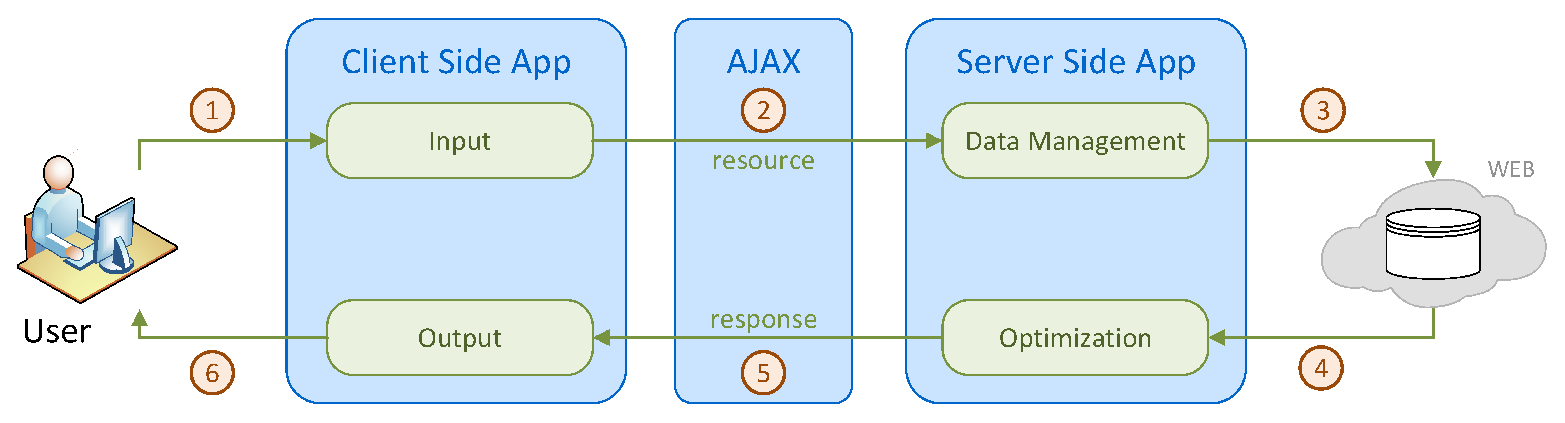
\includegraphics[width=1.0\columnwidth]{fig2.eps}
    \caption{Structure and data flow of the developed prototype.}
      \label{fig:system_architecture_design}  
\end{figure}

The response to a user request is not directly processed by the CSA, but rather by the Server-Side Application (SSA), which uses the issued parameters to produce a solution that minimizes the considered cost function. Such a solution  contains (at least) one set of flights that satisfy the user-defined request. Nonetheless, several other valid solutions may also be provided, to allow the user to choose the one that is more adequate to his needs. The most relevant information about each of the suggested flights is also provided (number 6), including:
\begin{itemize}
  \item the flight cost;
  \item the flight duration;
  \item the date, departure and arrival time;
  \item a hyperlink to a third-party API that allows a direct booking of the flight.
\end{itemize}

The developed CSA was implemented using the React JavaScript library (\url{www.reactjs.org}) and Redux framework (\url{www.reduxframework.com}), and the communication between the client and the server applications is done via Asynchronous JavaScript and XML (AJAX), which means that upon submitting the request (number 2), the user may continue to interact with the application until the SSA returns a response to the CSA (number 5).


\subsection{Server-Side Application}
\label{sec:ssa}

The SSA was implemented in a Python environment, together with Django framework (\url{www.djangoproject.com}). It comprises the following two main components: (i) a Data Management module, to fetch the flights data; and (ii) an Optimization module, which implements the devised search algorithms that find the best set of flights that satisfy the user request.


\subsubsection*{Data Management module}
\label{sec:ssa_data_management_system}

Since the issued user request only specifies an unordered list of trip nodes (i.e., the set of cities to be visited), the Data Management module is responsible for collecting all the flights information that is required to execute the devised optimization algorithms, thus completing the arcs (flights) that connect those nodes. Hence, an arc connecting two nodes corresponds to a flight between two cities, at a specific date. However, there are many flights that fit this description and each one may have several attributes that differentiate it from the others. For example, every flight has a particular cost, duration, departure and arrival time, airline company, bag limit or even different number of layover flights.

Due to the vast number of attributes that define every flight, it is impossible to know which particular flight is the most adequate for a specific user, because users often have different selection criteria. Hence, upon the construction of the multipartite graph, it makes sense to have a list of possible flights for every arc in $A$, instead of just a single one. This allows the selection of a specific flight according to the objective function being minimized. For example, if the goal is to minimize the total flight cost, it makes sense to select those flights that present the lowest cost, disregarding other attributes such as the airline company of the flights duration. This means that upon referring to an arc connecting two nodes, the Data Management module is actually considering a \textit{family} of arcs that share key characteristics (such as the origin, destination and date), but which may vary regarding other attributes.

To collect the data corresponding to each arc belonging to $A$, the developed system communicates with a third-party API and sends a request seeking the required flight objects. Among the several free and public flight-data APIs that might be used, it was adopted the API provided by the \textit{Kiwi} flight search company (\url{docs.kiwi.com}). 
Among the several useful features that are provided by this API is its ability to respond to a query over an extended search period. That is, upon requesting a flight between two cities, it is possible to specify a time window, instead of a single date. This is particularly useful because it allows the reduction of the total number of requests. While the total number of arcs in an FTP instance might be considerable, there is no need to make an individual request for every single arc. Instead, it is possible to submit a request for every pair of cities, by extending the search period to reflect the total number of necessary layers.

Having defined a complete graph, it is possible to run an optimization algorithm (number 4), in order to produce a valid solution to the user request. 


\subsubsection*{Optimization module}

The developed Optimization module implements the two considered metaheuristic algorithms: the Ant Colony Optimization and the Simulated Annealing. Both these algorithms require an initialization phase, which, among other things, defines some algorithm specific parameters. In order to inspect the same number of solutions in any given iteration of both algorithms, the number of ants ($m$) in the ACO was set the same as the Markov chain length ($M$) in the SA, which was initialized with the total number of nodes in $V$. Table~\ref{tab:parameters} summarizes the set of parameters used by the two metaheuristic algorithms of the implemented prototype.

\begin{table}[t]
\centering
\caption{Algorithm specific parameters.}
\label{tab:parameters}
\begin{tabular}{c l c}
\hline
Alg.                    &           Parameter                                            &       Value \\ \hline
\multirow{5}{*}{ACO}    &           Pheromone relative influence ($\alpha$)              &         1 \\
                        &           Heuristic relative influence ($\beta$)               &         5 \\
                        &           Pheromone evaporation rate ($\rho$)                  &       0.1 \\
                        &           Exploration rate ($Q_0$)                             &       0.9 \\ 
                        &           Number of ants ($m$)                                 & 10 \\ \hline
\multirow{6}{*}{SA}     &           First iter. acceptance prob. ($p_0$)                 & 0.98  \\ 
                        &           Last iter. acceptance prob. ($p_f$)                  & $10^{-300}$  \\
                        &           Initial temperature ($t_0$)                          & see Eq.~\ref{eq:t_zero} \\
                        &           Final temperature ($t_f$)                            & see Eq.~\ref{eq:cooling}  \\
                        &           Cooling parameter ($\lambda$)                        & see Eq.~\ref{eq:lambda} \\
                        &           Markov chain length ($M$)                            & $N$ \\ \hline
                         
\end{tabular}
\end{table}
%%%%%%%%%%%%%%%%%%%%%%%%%%%%%%%%%%%%%%%%%%%%%%%%%%%%%%%%%%%%%%%%%%%%%%%%%%%%%%%%%%%%%%%%%%%%%%%%%%%%%%%%%%%
%%%%%%%%%%%%%%%%%%%%%%%%%%%%%%%%%%%%%%%%%%%%%%%%%%%%%%%%%%%%%%%%%%%%%%%%%%%%%%%%%%%%%%%%%%%%%%%%%%%%%%%%%%%
\section{Experimental Results}
\label{sec:results}

In order to validate and evaluate the performance of the developed system, several tests were developed and executed. First, the implemented optimization algorithms are tested in order to evaluate their overall quality on a set of benchmarks. Then, the overall utility of the proposed and developed system is evaluated, by performing a series of tests on the Flying Tourist Problem. In particular, the quality of the obtained solutions are compared with those provided by the \textit{metric nearest neighbor} heuristic, which promotes the nodes proximity to define the traveling route and closely approximates the strategy usually adopted by a human solver. Finally, a thorough comparison with the only known state-of-the-art alternative for the devised FTP is performed by considering a comprehensive set of real-world multi-city formulations using different objective functions.

These experiments were executed on a 2.6GHz Intel i7-6700 CPU, with 8GB of RAM, and all the code was developed using the Python3 programming language. 


\subsection{Optimization module evaluation}

The main difficulty behind the aimed evaluation of the developed optimization module results from the absence of publicly available FTP benchmarks (with \textit{apriori} known optimal solutions) that could be used to validate the obtained results. To circumvent this adversity, it was decided to conduct such evaluation using closely-related NP-hard problems based on Asymmetric TSP and Time-Dependent TSP variations.


\subsubsection{Asymmetric TSP evaluation}

The set of benchmarks (and respective input data) that were considered for the Asymmetric TSP were collected from the publicly available TSPLib and correspond to problems with 17, 35, 53, 124 and 323 nodes (br17, ftv35, ft53, kro124p, rbg323, respectively). The adoption of such graph dimension ranges allows the evaluation of the developed optimization module with different complexity levels: small instances (17 nodes), corresponding to a dimension more closely-related to the targeted \textit{flying tourist} application scenario; medium instances (35-53 nodes), used to evaluate more computationally demanding scenarios; and large instances (124-323 nodes), used to evaluate the scalability of the developed system.

Each benchmark was independently solved by the two considered optimization algorithms (ACO and SA). The execution of each problem was repeated 5 times and the obtained results were averaged.  

Furthermore, since there are strict limitations on the maximum time a user is willing to wait for a result in a real-world application, it was considered a stop criteria to limit the total optimization time. In accordance, during the execution of these tests, each algorithm may run for no longer than 60 seconds. The results of both meta-heuristic algorithms on the considered set of asymmetric benchmarks are presented in Table~\ref{tab:tsp_results}. 

\begin{table}
    \centering
    \caption{Performance of the ACO and SA on the asymmetric TSP benchmarks, taken from the TSPLib (stop-criteria = 60 seconds). }
    \label{tab:tsp_results}
    \begin{tabular}{@{}l l c c c c c@{}}
    \hline
    \multirow{2}{*}{Alg.}& Bench   & \multirow{2}{*}{\#Iterat.}  & Optimal  & Comput.  & Error  \\ 
                         & mark    &                             & solution & solution &  [\%]  \\ \hline
    \multirow{5}{*}{ACO} & br17    & 6893    & 39        & 39       & 0              \\  
                         & ftv35   & 1469    & 1473      & 1552.4   & 5.39         \\  
                         & ft53    & 689     & 6905      & 8269.6   & 16.13        \\ 
                         & kro124p  & 275     & 36230     & 44102    & 17.00         \\   
                         & rbg323  & 20      & 1326      & 1660.4   & 25.21      \\ \hline
    \multirow{5}{*}{SA}  & br17    & 264319  & 39        & 39       & 0               \\  
                         & ftv35   & 63659   & 1473      & 1641		& 11.41       \\  
                         & ft53    & 36189   & 6905      & 7963     & 15.32        \\  
                         & kro124p  & 17533    & 36230     & 44102   & 21.73      \\  
                         & rbg323  & 1361    & 1326      & 1706.2   & 28.67        \\ \hline
    \end{tabular}
\end{table}

For small instances (17 nodes), both ACO and SA consistently present optimal solutions. For medium instances (35-53 nodes), both algorithms perform in the range of 5-16$\%$ relative error. As for bigger problems (124-323 nodes), the performance of the ACO slightly decreases (17-25\%), followed closely by the SA (22-29\%). 

By observing the number of iterations that were executed during the 60-seconds interval, it is clear that the SA is much faster than the ACO, performing 38 to 68 times more iterations in the same time period. However, this greater number of iterations does not seem to directly contribute for a better final result on the SA. This happens because the ACO search strategy is guided, taking into account the previous search experience in the selection of the next solution. This does not occur with the classical implementation of the SA, which utilizes a simple and non-guided local search.

On the other hand, while the considered stop-criteria value may be sufficient to reach the metaheuristic stationary result for small problem instances, meaning that continuing the optimization further may not affect the final error in a significant way, the higher relative error and lower number of iterations for bigger problem instances suggest that improvements may still occur.

To analyze the advantages of further optimization, all problems were solved once more, by using the same procedure previously described, this time for a total of 300 seconds. The obtained results are presented in Table~\ref{tab:further_opt}, which allow the comparison of the final result as a function of the execution time. Columns RE60 and RE300 present the relative error after 60 and 300 seconds, respectively. As it can be seen, increasing the optimization time leads to an improvement in the final result for both metaheuristics and for almost every problem. These improvements are more significant for bigger problems and affect the small instances only slightly.

Hence, the observed performance of the implemented metaheuristic algorithms on the asymmetric TSP for the level of complexity of the targeted \textit{flying tourist} application scenario showed to be highly promising, leading to final solutions which are either optimal or whose relative error is close to 10\%. 

\begin{table}[t]
\centering
\caption{Effects of increased optimization time on the final result.}
\label{tab:further_opt}
\begin{tabular}{ccccc}
\hline
         & \multicolumn{2}{c}{ACO} & \multicolumn{2}{c}{SA} \\
Benchmark & RE60      & RE300      & RE60       & RE300      \\ \hline
br17     & 0          & 0          & 0         & 0          \\
ftv35    & 5.39       & 4.75           & 11.41     & 11.73      \\
ft53     & 16.13      & 13.71 			& 15.32     & 13.20      \\
kro124p   & 17.00       & 13.91            & 21.73     & 17.21      \\
rbg323   & 25.21      & 18.78            & 28.67     & 10.27      \\
\hline
\end{tabular}
\end{table}


\subsubsection{Time-dependent TSP evaluation}

Due to the absence of standardized benchmarks for the time-dependent case in the TSPLib, it was necessary to define specific problems (whose best known solutions are known \textit{apriori}) by using a method described in (\cite{TDTSP_construction}), based on the duality principle over the Integer Linear formulation for the time-dependent TSP. The defined benchmarks were based on those used for the Asymmetric TSP and their names were appended with an asterisk suffix to distinguish from the original ones.

Executing the same evaluation strategy on the time-dependent TSP problems leads to the results presented in Table~\ref{tab:tdtsp_results}. Once again, it is possible to compare the efficiency of the ACO and the SA, by evaluating the relative error of each set of problems.

\begin{table}
    \centering
    \caption{Performance of the ACO and SA on the time-dependent TSP benchmarks (stop-criteria = 60 seconds).}
    \label{tab:tdtsp_results}
    \begin{tabular}{@{}l l@{}c c c c c@{}}
    \hline
    \multirow{2}{*}{Alg.}& Bench   & \multirow{2}{*}{\#Iterat.}  & Optimal  & Comput.  & Error  \\ 
                         & mark    &                             & solution & solution &  [\%]  \\ \hline
    \multirow{5}{*}{ACO} & br17*    & 9720    & 2458        & 2729                 & 11.03          \\  
                         & ftv35*   & 2590    & 5131       & 5500              & 7.20       \\  
                         & ft53*    & 1099     & 7930      & 8370               & 5.53      \\ 
                         & kro124p*  & 71     & 25483     & 26402         & 3.61     \\   
                         & rbg323*  & 13      & 48991      & 50261                & 2.59      \\ \hline
    \multirow{5}{*}{SA}  & br17*    & 219517  & 2458        & 2631             & 7.04          \\  
                         & ftv35*   & 80262   & 5131      & 5406			  & 5.38      \\  
                         & ft53*    & 37450   & 7930      & 8265           & 4.23      \\  
                         & kro124p*  & 3521    & 25483     & 26427         & 3.70     \\  
                         & rbg323*  & 901    & 48991      & 51926              & 5.99      \\ \hline
    \end{tabular}
\end{table}

For small instances (17 nodes), ACO and SA present a small relative error, ranging from 7\% and 11\%. For medium instances (35-53 nodes), the relative error decreases for both algorithms, ranging from 4\% to 7\%, with SA offering better results than ACO. This may occur because the high number of performed iterations in small and medium instances leads to an intensive search space exploration. However, when  bigger problems (124-323 nodes) are considered, the performance of the ACO increases (possibly due to its guided search exploration), reducing the relative error to close to 3\% and surpassing that of the SA.

In any case, the performance of these two algorithms on the time-dependent TSP is highly promising, leading to final solutions which are consistently below the 10\% relative error mark. 


\subsubsection{Discussion}

A precise interpretation of the factors involved in these results is not straightforward. Still, the following conclusions seem plausible. When comparing the time-dependent TSP with the asymmetric TSP, the former is usually expected to be more heavily constrained than the latter. In those cases, finding the problem itself simplifies the search for the overall optimum, as bad solutions are much easier to identify. In particular, both ACO and SA seem to explore this property well, as it can be inferred by the fact that for the corresponding benchmarks, the time dependent version obtains a better relative error rate with less iterations. Moreover, the better relative error rates themselves seem to be problem induced, meaning that the asymmetric TSP contains big gaps in the objective function. This happens, in particular, from the optimal value to a close by maximum, whereas the time-dependent TSP contains smaller gaps and a higher concentration of near maximums.


\subsection{Flying Tourist Problem evaluation}

To demonstrate and quantify the actual benefits of the proposed system, a series of FTP instances were defined, ranging from just 1 city to visit (which corresponds to a round-way flight), up to a total of 20 cities. For each problem instance, several solutions were obtained using four different approaches:
\begin{itemize}
    \item a \textit{pseudo-random} approach, i.e., a closed trip randomly generated that connects the cities;
    \item a \textit{metric nearest-neighbor} heuristic that promotes the nodes proximity to define the traveling route (this straightforward approach closely approximates the strategy usually followed by a human solver);
    \item a \textit{regular nearest-neighbor} heuristic using the flight price as the objective function;
    \item the \textit{proposed ACO and SA} meta-heuristics (where the best of these two results is chosen), considering two different objective functions (minimization of the total cost and of the entropy).
\end{itemize}  

In this experiment, the number of nodes was varied and multiple requests (more than 5) were made for each set of nodes, averaging their results. In every case, the trip starts and returns to Lisbon (Portugal) and visits a given set of cities, randomly chosen from the following set: Abuja, Atlanta, Barcelona, Beijing, Cairo, Casablanca, Dubai, Dublin, Frankfurt, Hong Kong, Istanbul, Johannesburg, Kiev, Los Angeles, Madrid, Miami, Moscow, New-York (JFK), Oslo, San Francisco, Sidney, Singapore. The start date was set to be the same for all requests(\textit{1 November 2018}), which, upon the execution of the tests, was 50 days into the future. The waiting period on each city was set to a random value between 1 and 5 days. 


\subsubsection{Quantitative evaluation and improvement}

\begin{table*}
    \definecolor{Gray}{gray}{0.9}
    \definecolor{green}{rgb}{0,0.5,0}
    \definecolor{red}{rgb}{0.75,0,0}
    \setlength\tabcolsep{4pt}
    \renewcommand{\arraystretch}{1.25}
    \centering
    \caption{Comparison of different Flying Tourist Problem solutions obtained with distinct algorithms and optimization criteria, considering the \textit{Metric Nearest Neighbor} approach (shaded gray) as reference.} 
    \resizebox{1.0\textwidth}{!}{
      \begin{tabular}{l|l|r@{~}r|r@{~}r|r@{~}r|r@{~}r|r@{~}r|r@{~}r|r@{~}r|}
      \label{tab:utility}
                                         & \multicolumn{1}{r}{\#Nodes} 
                                         & \multicolumn{2}{|c}{1} 
                                         & \multicolumn{2}{|c}{3}    
                                         & \multicolumn{2}{|c}{5}    
                                         & \multicolumn{2}{|c}{7}
                                         & \multicolumn{2}{|c}{10}   
                                         & \multicolumn{2}{|c}{15}
                                         & \multicolumn{2}{|c|}{20}   \\
      \hline  
      \multirow{4}{*}{\begin{sideways}\hspace*{-4ex}\textbf{PRICE}\end{sideways}}     
                        & Random            & 635  & 
                                                    & 1455 & {\color{red}(+1.2\%)} 
                                                    & 2194 & {\color{red}(+7.0\%)} 
                                                    & 3436 & {\color{red}(+26.6\%)} 
                                                    & 4791 & {\color{red}(+28.8\%)} 
                                                    & 7222 & {\color{red}(+63.5\%)} 
                                                    & 9154 & {\color{red}(+68.8\%)} \\
                        & \cellcolor{Gray}Metric Nearest Neighbor   
                                                    & \cellcolor{Gray}635  & \cellcolor{Gray}
                                                    & \cellcolor{Gray}1438 & \cellcolor{Gray}
                                                    & \cellcolor{Gray}2051 & \cellcolor{Gray}
                                                    & \cellcolor{Gray}2715 & \cellcolor{Gray}
                                                    & \cellcolor{Gray}3721 & \cellcolor{Gray}
                                                    & \cellcolor{Gray}4417 & \cellcolor{Gray}
                                                    & \cellcolor{Gray}5422 & \cellcolor{Gray} \\
                        & Regular Nearest Neighbor  & 635  & 
                                                    & 1438 & 
                                                    & 1993 & {\color{green}(-2.8\%)} 
                                                    & 2553 & {\color{green}(-6.0\%)}
                                                    & 3412 & {\color{green}(-8.3\%)}
                                                    & 3911 & {\color{green}(-11.5\%)}
                                                    & 4678 & {\color{green}(-13.7\%)} \\
                                & Proposed (Price)   & 635  & 
                                                    & 1398 & {\color{green}(-2.8\%)}
                                                    & 1727 & {\color{green}(-15.8\%)}
                                                    & 1911 & {\color{green}(-29.6\%)}
                                                    & 2466 & {\color{green}(-33.7\%)}
                                                    & 3051 & {\color{green}(-30.9\%)}
                                                    & 3699 & {\color{green}(-31.8\%)} \\
                                & Proposed (Entropy)& 876 & {\color{red}(+38.0\%)} 
                                                    & 1761 & {\color{red}(+22.5\%)}
                                                    & 2203 & {\color{red}(+7.4\%)}
                                                    & 2749 & {\color{red}(+1.3\%)}
                                                    & 3687 & {\color{green}(-0.9\%)}
                                                    & 4123 & {\color{green}(-6.7\%)}
                                                    & 4707 & {\color{green}(-13.2\%)} \\ \hline
      \multirow{4}{*}{\begin{sideways}\hspace*{-4ex}\textbf{DURATION}\end{sideways}} 
                                & Random            & 61   & 
                                                    & 125  & {\color{red}(+5.0\%)} 
                                                    & 183  & {\color{red}(+3.4\%)} 
                                                    & 270  & {\color{red}(+31.7\%)} 
                                                    & 369  & {\color{red}(+48.2\%)} 
                                                    & 497  & {\color{red}(+63.0\%)} 
                                                    & 638  & {\color{red}(+92.7\%)}  \\
                                & \cellcolor{Gray}Metric Nearest Neighbor        
                                                    & \cellcolor{Gray}61 & \cellcolor{Gray}
                                                    & \cellcolor{Gray}119 & \cellcolor{Gray}
                                                    & \cellcolor{Gray}177 & \cellcolor{Gray}
                                                    & \cellcolor{Gray}205 & \cellcolor{Gray}
                                                    & \cellcolor{Gray}249 & \cellcolor{Gray}
                                                    & \cellcolor{Gray}305 & \cellcolor{Gray}
                                                    & \cellcolor{Gray}331 & \cellcolor{Gray}  \\
                                & Regular Nearest Neighbor       & 61 & 
                                                    & 119 & 
                                                    & 181 & {\color{red}(+2.3\%)}
                                                    & 212 & {\color{red}(+3.4\%)}
                                                    & 257 & {\color{red}(+3.2\%)}
                                                    & 323 & {\color{red}(+5.9\%)}
                                                    & 358 & {\color{red}(+8.2\%)}  \\
                                & Proposed (Price)   & 61 & 
                                                    & 121 & {\color{red}(+1.7\%)}
                                                    & 151 & {\color{green}(-14.7\%)}
                                                    & 179 & {\color{green}(-12.7\%)}
                                                    & 258 & {\color{green}(+3.6\%)}
                                                    & 292 & {\color{green}(-4.3\%)}
                                                    & 319 & {\color{green}(-3.6\%)}  \\
                                & Proposed (Entropy)& 29 & {\color{green}(-52.5\%)}
                                                    & 57 & {\color{green}(-52.1\%)}
                                                    & 82 & {\color{green}(-53.7\%)}
                                                    & 92 & {\color{green}(-55.1\%)}
                                                    & 104 & {\color{green}(-58.2\%)}
                                                    & 140 & {\color{green}(-54.1\%)}
                                                    & 160 & {\color{green}(-51.7\%)} \\ \hline 
      \end{tabular}
    }
\end{table*}

The result of the execution of the described test is summarized in Table~\ref{tab:utility}, where both the total flight cost and duration are presented, as a function of the optimization approaches and the number of nodes. This table also presents the observed improvement, relative to the \textit{metric nearest-neighbor} solution, used as reference.

The first insight into these results allows a preliminary evaluation of the utility of the proposed system. It can be seen that, for a small number of nodes (1 and 3), there is no significant improvement relative to the \textit{metric nearest-neighbor} solution. However, when greater instances (5-20 nodes) are considered, this straightforward approach stops presenting good results, while its regular variant (using the flight prices objective function) and the proposed meta-heuristics greatly improve the total flights cost ($\approx$ 3-34\%). However, despite the good results that were presented by the regular nearest neighbour approach (using the flight prices), the proposed meta-heuristics are still capable of improving them ($\approx$ 3-25\%).    


\subsubsection{Balancing the total flight price and duration}

Another implementation of the proposed metaheuristics was also considered that introduce the flight duration in the objective function. With such an alternative implementation, it was envisaged a better balance between price and flight duration, by minimizing an entropy metric defined as a weighted value where the price and flight duration contribute with 70\% and 30\%, respectively.

As it can be observed in Table~\ref{tab:utility}, such an entropic minimization leads to significant improvements in the flight duration, although it introduces some penalization in the flight price for a small number of nodes (1-5). However, as the number of nodes increases, the flight price significantly decreases, but it is always higher than that provided by the former price-only meta-heuristics. This happens because the two objective functions (price and duration) can hardly be simultaneously minimized, and thus, a compromise has to be reached. In this case, compromising means slightly increasing the price, to significantly reduce the duration.

This compromise between flight price and duration is also illustrated in Fig.~\ref{fig:cost_vs_time}, which presents the relative duration improvement as a consequence of the increase in price. This figure shows that, in general, increasing the price by around 20\% leads to a decrease in the flight duration by around 50\%, when compared to the price-only metaheuristic.

\begin{figure}
  \centering
  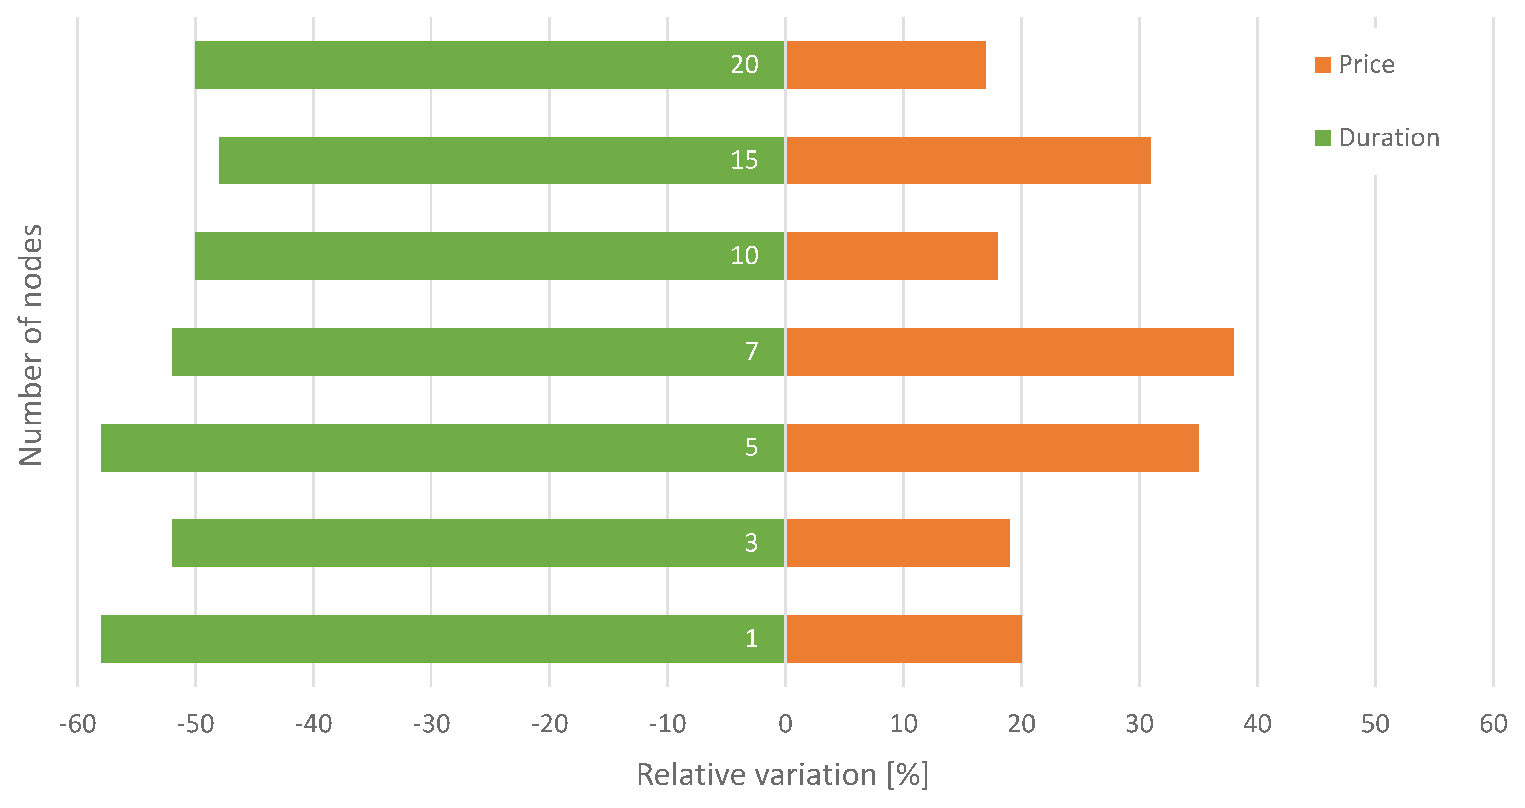
\includegraphics[width=1.0\columnwidth]{fig3.eps}
  \caption{Variation of the total flight price and duration when minimizing the entropy objective function.}
  \label{fig:cost_vs_time}  
\end{figure}


\subsubsection{Impact of the trip start interval}

To evaluate the influence of the trip start interval on the obtained results, the same queries and data sets were used to solve these FTPs using start periods of different lengths. These results are illustrated in Fig.~\ref{fig:cost_vs_startperiod}, where $NN$ refers to the \textit{metric nearest neighbour} heuristic and $M-1$, $M-15$ and $M-31$ represents the proposed meta-heuristic algorithms, with start periods of length 1, 15 and 31 days, respectively. 

The analysis of Fig.~\ref{fig:cost_vs_startperiod} shows that increasing the interval of the start date may lead to even greater benefits, with flight price improvements as high as 15\%.  

\begin{figure}[t]
  \centering
  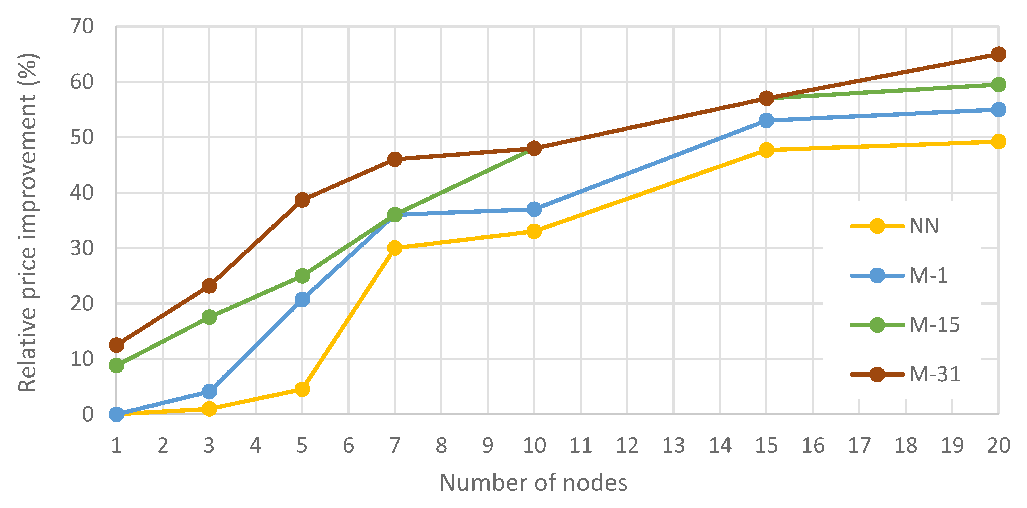
\includegraphics[width=1.0\columnwidth]{fig4.eps}
  \caption{Price improvement as a function of the trip start interval.}
  \label{fig:cost_vs_startperiod}  
\end{figure}


\subsubsection{Response time}

The response time of any query depends of two different procedures: the data gathering and the optimization. In this case, the optimization time is mostly constant and established \textit{apriori}. In contrast, the data gathering is usually the bottleneck of the process, because the construction of the cost matrix requires massive amounts of data. 

The total time that is necessary to respond to a request, as a function of the number of nodes and length of the start interval, is illustrated in Fig.~\ref{fig:response_time}. From the analysis of this figure, it can be seen that requests with up to 10 nodes can be solved in less than 60 seconds. It can also be seen that the response time increases non-linearly as the number of nodes increases. On the other hand, increasing the length of the start interval has low influence for small instances (up to 10 nodes), but has a significant impact for greater instances.

\begin{figure}
  \centering
  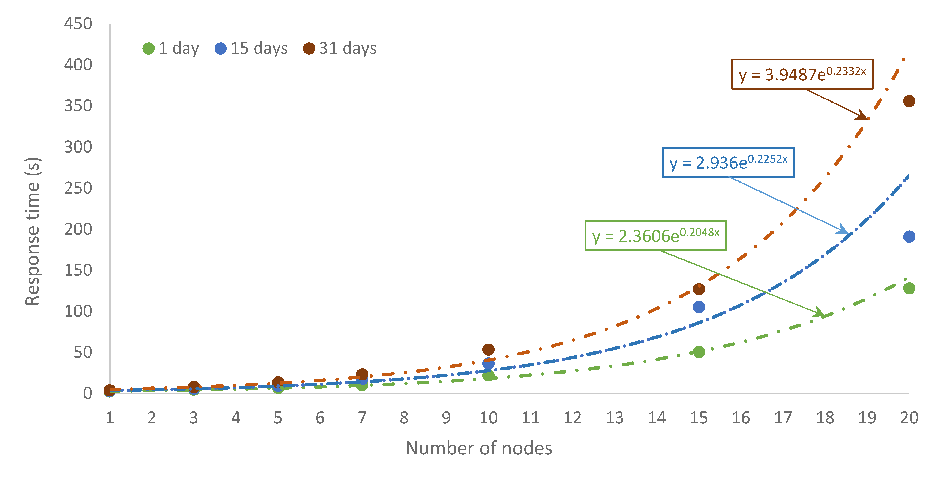
\includegraphics[width=1.0\columnwidth]{fig5.eps}
  \caption{Total response time to a request, as a function of the number of nodes and length of start period.}
  \label{fig:response_time}  
\end{figure}


\subsection{Comparison with \textit{Kiwi}'s \textit{Nomad}}

At the present time, \textit{Kiwi}'s \textit{Nomad} is the only (non-disclosed) tool that is capable of addressing the formalized \textit{Flying Tourist Problem} in the form of an unconstrained multi-city routing problem, although limited to only 10 different nodes. To facilitate the comparison of the conceived optimization system with this tool, the definition of the user requests of the proposed FTP (see section \ref{sec:problem}) was kept as similar as possible to \textit{Kiwi}'s \textit{Nomad} interface. The user is asked to specify the departing/arriving city, together with the start date, the set of cities to be visited and the duration of the stay in each city.

The results provided by both applications were extensively compared against each other, according to each considered objective function. The difference in the total flight price and duration (for each query) was also measured and analyzed as a function of the query parameters. The former evaluation will be called \textit{absolute comparison}, while the latter \textit{quantative evaluation}.

The execution of these tests involved over 100 different queries, by varying not only the number of nodes (2-10), but also the length of the trip start interval (1-15 days). All queries that were performed on both applications had its start and return city set to Lisbon (Portugal), while each city to be visited belongs to the same set of hub airports that were considered in the previous subsections. These queries were executed during the period between 15 and 16 of June 2018 and the base start date was set to the 1st of August 2018, which, at the time of the tests, was 45 days in the future. The staying period in each city was set to a random value between 1 and 5 days. For extended start periods, the base start date was extended by 31 days.


\subsubsection{Absolute comparison}

Both applications respond to each query with three different sets of flights, serving the following different optimization criteria: the \textit{cheapest}, the \textit{fastest} and the \textit{recommended}. For each query, a winner was determined according to these criteria. The cheapest set of flights is determined according to the total flight price, while the fastest depends solely on the total flight duration. The recommended set of flights depends on both the price and the duration, and the winner for this criteria must have both lower prices and duration. 

\begin{figure}
    \centering
    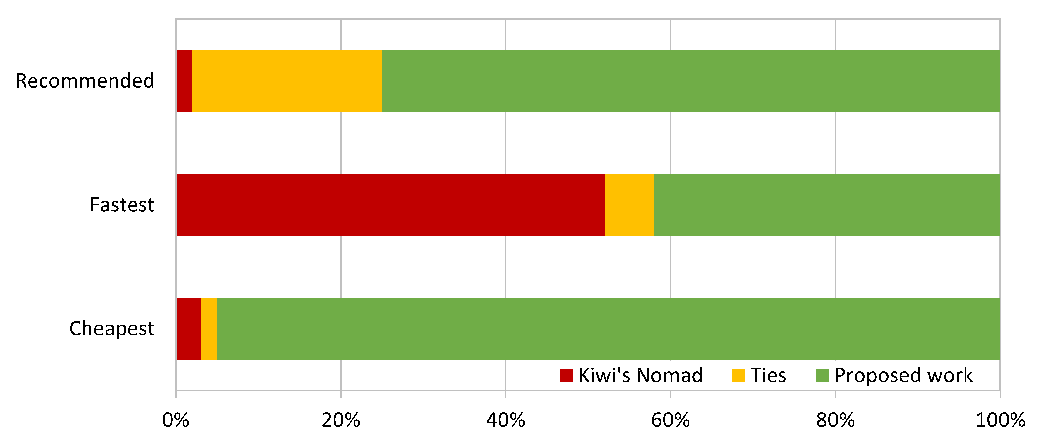
\includegraphics[width=1.0\columnwidth]{fig6.eps}
    \caption{Comparison of the results provided by the proposed tool and by \textit{Kiwi}'s \textit{Nomad} application.}
    \label{fig:quality_apis}
\end{figure}

Fig.~\ref{fig:quality_apis} illustrates the obtained comparison, by presenting the total number of times that an application outperformed the other, for each of the three different optimization criteria. It also shows the number of cases in which the responses were very similar.

The analysis of this figure indicates that the developed application presents better solutions for a significant amount of queries. In fact, while the fastest set of flights is only achieved in 42\% of the queries, it presents the cheapest set of flights 95\% of the times and the best recommended result 75\% of the times.  


\subsubsection{Quantitative evaluation}

To evaluate the difference of the responses provided by both applications, the total flight price and duration of the recommended set of flights was also quantitatively measured (see Fig.~\ref{fig:comparison}). The values presented in these graphs refer to the developed application response and were normalized using the \textit{Kiwi}'s \textit{Nomad} response as reference. 

\begin{figure}[!ht]
    \centering
    \begin{subfigure}[a]{1\columnwidth}
      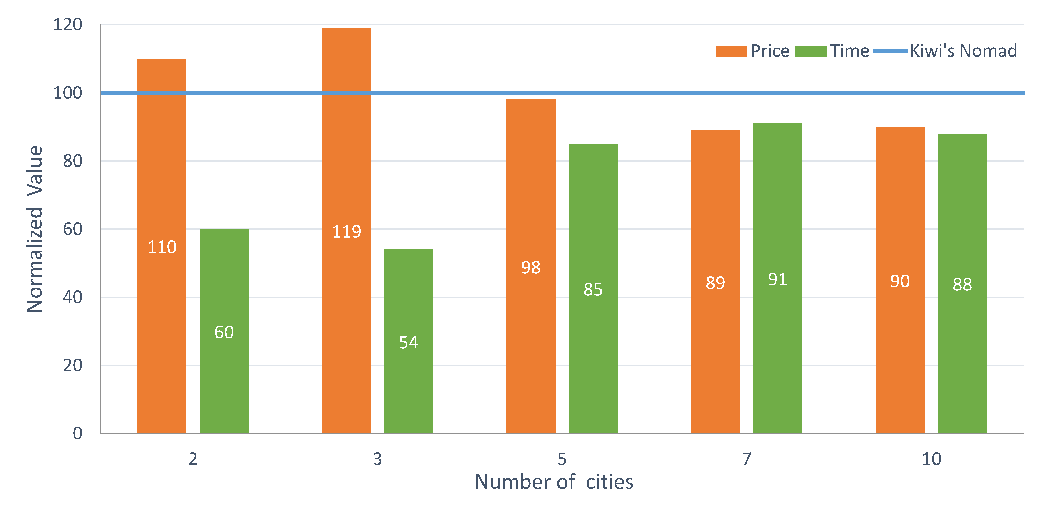
\includegraphics[width=1\columnwidth]{fig7a.eps}
      \caption{Single start date.}
      \label{fig:comparison_a} 
    \end{subfigure}
    \begin{subfigure}[b]{1\columnwidth}
      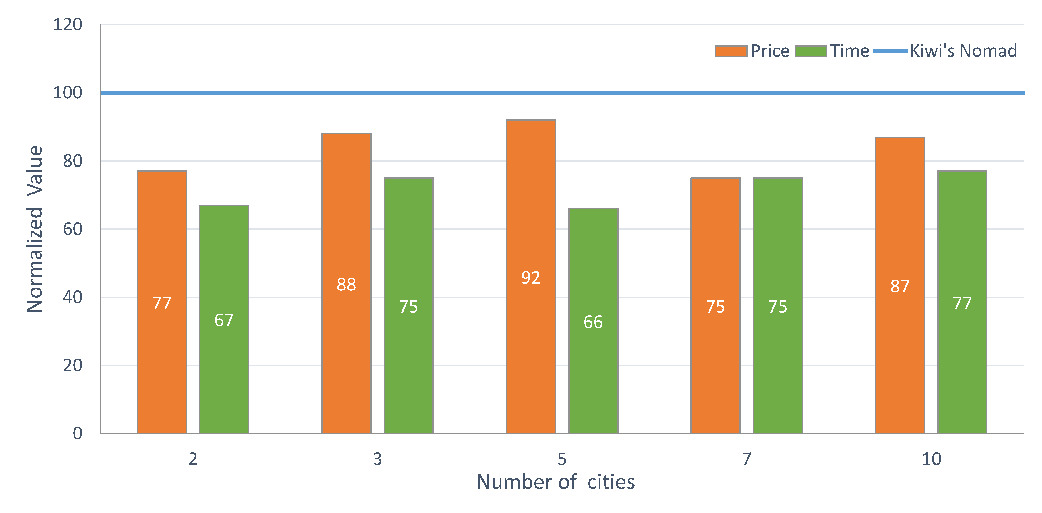
\includegraphics[width=1\columnwidth]{fig7b.eps}
      \caption{Extended start period (31 days).}
      \label{fig:comparison_b}
    \end{subfigure}
 \caption{Comparison of the recommended flights price and duration, as a function of the number of nodes and the length of start interval. The presented values refer to the proposed application response, and were normalized with respect to \textit{Kiwi}'s \textit{Nomad} response value.}
 \label{fig:comparison}
\end{figure}

Fig.~\ref{fig:comparison_a} presents the results of the queries performed for a single start date. Its analysis shows that, for a small number of nodes (2 and 3), the developed application recommends flights that are slightly more expensive (10 to 19\%) than those presented by \textit{Kiwi}. In contrast, the flight duration of these flights is much lower (33-46\%). For requests with more nodes (5 to 10), the results presented by the developed application have both lower prices (2-18\%) and flight duration (9-24\%). Fig.~\ref{fig:comparison_b} depicts the obtained results when the length of the start interval was extended to 31 days. With such an extended start period, every recommended set of flights provided by the proposed application has a lower price and duration. The price presents the most significant change: the minimum improvement is 8\%, while the maximum is 29\%.

Finally, it is worth noting that all the presented experiments only consider up to 10 different cities to be visited by the traveler. The reason why more nodes were not considered arises not from the developed application (which could easily accommodate more cities), but is motivated by a strict limit presented by \textit{Kiwi}'s \textit{Nomad} user interface, which does not support more than 10 nodes in the planned route.

%%%%%%%%%%%%%%%%%%%%%%%%%%%%%%%%%%%%%%%%%%%%%%%%%%%%%%%%%%%%%%%%%%%%%%%%%%%%%%%%%%%%%%%%%%%%%%%%%%%%%%%%%%%
%%%%%%%%%%%%%%%%%%%%%%%%%%%%%%%%%%%%%%%%%%%%%%%%%%%%%%%%%%%%%%%%%%%%%%%%%%%%%%%%%%%%%%%%%%%%%%%%%%%%%%%%%%%
\section{Conclusions}
\label{sec:conclusions}
Despite the existence of numerous flight search applications, most of them lack the ability to properly address unconstrained multi-city flight requests, since this problem is generally not tractable. To circumvent this absence, the presented work formalizes and addresses the Flying Tourist Problem (FTP), a NP-hard problem that occurs as a generalization of the Traveling Salesman Problem (TSP), and whose goal is to find the best schedule, route, and set of flights, for an unconstrained multi-city flight request.

An effective methodology that allows an efficient resolution of this rather demanding problem was proposed, based on different heuristics and meta-heuristic optimization algorithms, including the Ant Colony Optimization and the Simulated Annealing, allowing the identification of solutions in real-time, even for large instances. The developed methods were integrated into a web application prototype, allowing a fast resolution of user-defined requests. 

The implemented system was evaluated using different criteria, including the quality of its optimization system; the utility of the devised problem; and its performance compared to other similar systems. The obtained results show that the developed optimization system consistently presents solutions that are as close as 10\% to the optimal value and the considered meta-heuristic optimization strategies present solutions that are up to 35\% cheaper than those developed by simpler heuristics. Furthermore, when comparing the developed system to the only known (but not-disclosed) alternative, it was shown that it provides the cheapest and the best-recommended solutions, respectively 95\% and 74\% of the times. 

As a result, upon the planning of a complex multi-city trip, the developed system showed to allow the user to save a significant amount of time and money.
%%%%%%%%%%%%%%%%%%%%%%%%%%%%%%%%%%%%%%%%%%%%%%%%%%%%%%%%%%%%%%%%%%%%%%%%%%%%%%%%%%%%%%%%%%%%%%%%%%%%%%%%%%%
%%%%%%%%%%%%%%%%%%%%%%%%%%%%%%%%%%%%%%%%%%%%%%%%%%%%%%%%%%%%%%%%%%%%%%%%%%%%%%%%%%%%%%%%%%%%%%%%%%%%%%%%%%%
\section*{Acknowledgements}
This work was partially supported by national funds through Funda\c{c}\~ao para a Ci\^encia e a Tecnologia (FCT) under project UID/CEC/50021/2019.
%%%%%%%%%%%%%%%%%%%%%%%%%%%%%%%%%%%%%%%%%%%%%%%%%%%%%%%%%%%%%%%%%%%%%%%%%%%%%%%%%%%%%%%%%%%%%%%%%%%%%%%%%%%
%%%%%%%%%%%%%%%%%%%%%%%%%%%%%%%%%%%%%%%%%%%%%%%%%%%%%%%%%%%%%%%%%%%%%%%%%%%%%%%%%%%%%%%%%%%%%%%%%%%%%%%%%%%

%\section*{Bibliography}
%% References
%%
%% Following citation commands can be used in the body text:
%% Usage of \cite is as follows:
%%   \cite{key}          ==>>  [#]
%%   \cite[chap. 2]{key} ==>>  [#, chap. 2]
%%   \citet{key}         ==>>  Author [#]

%% References with bibTeX database:

%\bibliographystyle{model1-num-names}
\bibliographystyle{elsarticle-harv.bst}\biboptions{round,authoryear}

\bibliography{ftp_RMarques.bib}

%% Authors are advised to submit their bibtex database files. They are
%% requested to list a bibtex style file in the manuscript if they do
%% not want to use model1-num-names.bst.

%% References without bibTeX database:

% \begin{thebibliography}{00}

%% \bibitem must have the following form:
%%   \bibitem{key}...
%%

% \bibitem{}

% \end{thebibliography}


\end{document}
